\documentclass[a4paper, oneside]{book}
\usepackage[T1]{fontenc}
\usepackage[utf8]{inputenc}
\usepackage[latin1]{inputenc}
\usepackage[italian]{babel}
\usepackage{graphicx}	
\usepackage{makeidx}
\usepackage{hyperref}
\usepackage{color}
\usepackage[labelfont=bf]{caption}
\usepackage{amssymb}
\usepackage{listings}
\usepackage{midpage}
\usepackage[margin=1.1in]{geometry}



\makeindex
\lstset{language=Java, frameround=fttt, breaklines=true, showstringspaces=false, 
	basicstyle=\scriptsize\ttfamily, keywordstyle=\color{blue}\bfseries, stringstyle=\color{gray}, commentstyle=\color{green}}

\pagestyle{empty} 

\begin{document}


% Logo e nome facoltà
\large
\begin{figure}
	\begin{center}
		
\includegraphics[scale=0.30]{logo_parthenope.png} \\
		\textsc{Università degli Studi di Napoli Parthenope \\	
	        	Dipartimento di Scienze e Tecnologie \\
		        Corso di programmazione III}
            		   \rule{\textwidth}{0.9mm}
            		   \footnote{Giuseppe Accardo - 0124000879}
	\end{center}
\end{figure}

% Logo progetto
\begin{center}
\Huge{\bfseries\textcolor{blue}{{  Data Mining}}} \\
        \vspace{0.3cm}

        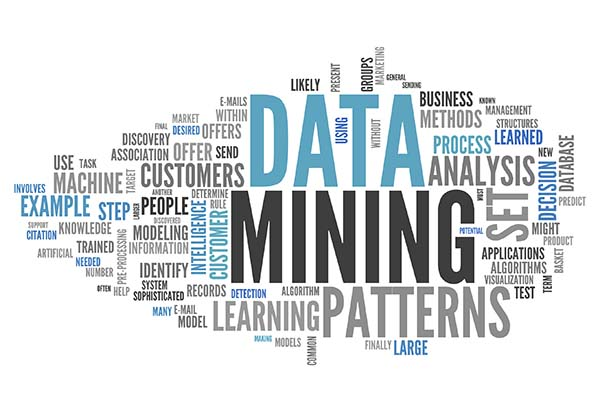
\includegraphics[scale=2.60]{FotoProgetto.jpg} \\
        \vspace{0.7cm}
\end{center}


% Dati studente
\begin{center}
	\large\textbf{\textsc{Titolo Progetto}} {  Data Mining} \\ \vspace{0.35cm}
	\large\textbf{\textsc{Studente:}} {Giuseppe Accardo} \\  
	\vspace{0.3cm}
	\large\textbf{\textsc{Matricola:}} { 0124000879} \\ 
	\vspace{0.3cm}
	\large\textbf{\textsc{Anno Accedemico:}} {2016/2017} \\
	\vspace{0.3cm}
	\large\textbf{\textsc{Docente:}} {Angelo Ciaramella} \\
\end{center}


\newpage

% Indice delle tabelle
\newpage
\begingroup 
\let\clearpage\relax
	\let\cleardoublepage\relax
	\par\vspace{2\baselineskip}
		
\tableofcontents 
 \endgroup 

       
       
\pagestyle{myheadings} 
\markboth{\MakeUppercase{Traccia e descrizione del problema}}{\MakeUppercase{Traccia e descrizione del problema}}\chapter*{Traccia e descrizione del problema}
\addcontentsline{toc}{chapter}{Traccia e descrizione del problema}
\pagestyle{myheadings} 

\large
\section*{Problema}
\addcontentsline{toc}{section}{Problema}
Si vuole sviluppare un sistema di \textbf{Data Mining} per l'elaborazione di dati. Il Data Mining comprende un insieme di tecniche e metodologie che hanno per oggetto l'estrazione e visualizzazione di informazioni da grandi quantit`a di dati. Le fasi principali del sistema che si vuole sviluppare sono: \textbf{selezione delle caratteristiche, clustering e visualizzazione}.\\
Si suppone di avere un data set contnuto in un file .data. Il data set `e ralativo alla classificazione di 3 tipi di rose (setosa, versicolour, virginica) mediante sue quattro carattrisiche (feature): lunghezza e larghezza del sepalo, lunghezza e larghezza del petalo.\\
Nella fase di selezione delle caratteristiche un utente pu`o scegliere il numero di caratteirstiche da selezionare per l'analisi (le colonne del data set).
Nella fase di clustering viene usato un algoritmo per “agglomerare” dati simili. Nel caso specifico viene usato l'algoritmo K-Means. L'utente pu`o scegliere il numero di “cluster” da usare.\\
Nella fase di visualizzazione i dati “agglomerati” sono visualizzati in 2 e 3 dimensioni. Nel caso in cui il numero delle feature `e piu` grande di 3 viene applicato un algoritmo di Analisi delle Componenti Principali per la visualizzazione.
\\
\large
\newpage
\section*{Cos'è il Datamining}
\addcontentsline{toc}{section}{Cos'è il Datamining}
Il \textbf{data mining} è l'insieme di tecniche e metodologie che hanno per oggetto l'estrazione di un sapere o di una conoscenza a partire da grandi quantità di dati (attraverso metodi automatici o semi-automatici) e l'utilizzo scientifico, industriale o operativo di questo sapere. \\
e tecniche di data mining sono fondate su specifici algoritmi. I pattern identificati possono essere, a loro volta, il punto di partenza per ipotizzare e quindi verificare nuove relazioni di tipo causale fra fenomeni; in generale, possono servire in senso statistico per formulare previsioni su nuovi insiemi di dati.\\
Un concetto correlato al data mining è quello di apprendimento automatico (\textbf{Machine learning}); infatti, l'identificazione di pattern può paragonarsi all'apprendimento, da parte del sistema di data mining, di una relazione causale precedentemente ignota, cosa che trova applicazione in ambiti come quello degli algoritmi euristici e dell'intelligenza artificiale. Tuttavia, occorre notare che il processo di data mining è sempre sottoposto al rischio di rivelare relazioni causali che poi si rivelano inesistenti.\\
In questo caso si utilizzerà la tecnica del Clustering mediante l'applicazione dell'algoritmo K-Means, un algoritmo del tipo "unsupervised classification" poichè le classi modello non vengono definite dall'utente, ma vengono ricostruite automaticamente. L'utente decide solo il numero di gruppi. Lo scopo del sistema sarà di "riconoscere" le rose in base alle loro caratteristiche.
\begin{figure}[htp]
\centering
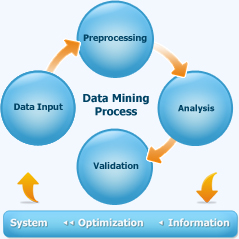
\includegraphics[width=10cm]{datamining.jpg}
\caption{Datamining}
\label{fig:Datamining}
\end{figure}

\newpage
\large
\section*{Struttura del Dataset}
\addcontentsline{toc}{section}{Struttura del Dataset}
Un \textbf{dataset} (o data set) è una collezione di dati.\\
Più comunemente un dataset costituisce un insieme di dati strutturati in forma relazionale, cioè corrisponde al contenuto di una singola tabella di database, oppure ad una singola matrice di dati statistici, in cui ogni colonna della tabella rappresenta una particolare variabile, e ogni riga corrisponde ad un determinato membro del dataset in questione.\\
La dimensione del dataset è data dal numero dei membri presenti (\textbf{osservazioni)}, che formano le righe, e dal numero delle variabili di cui si compone (\textbf{features}), che formano le colonne.
\\
\large
\subsection*{Dataset Iris}
 \addcontentsline{toc}{subsection}{Dataset Iris}
Il dataset Iris è un dataset multivariato introdotto da Ronald Fisher nel 1936. Consiste in 150 istanze di Iris misurate da Edgar Anderson e classificate secondo tre specie: Iris setosa, Iris virginica e Iris versicolor. Le quattro variabili considerate sono la lunghezza e la larghezza del sepalo e del petalo. A causa di errori, esistono diverse versioni del dataset utilizzate nella letteratura scientifica.
Il dataset Iris viene utilizzato nell'ambito dell'apprendimento automatico come esempio di classificazione statistica.
\begin{figure}[htp]
\centering
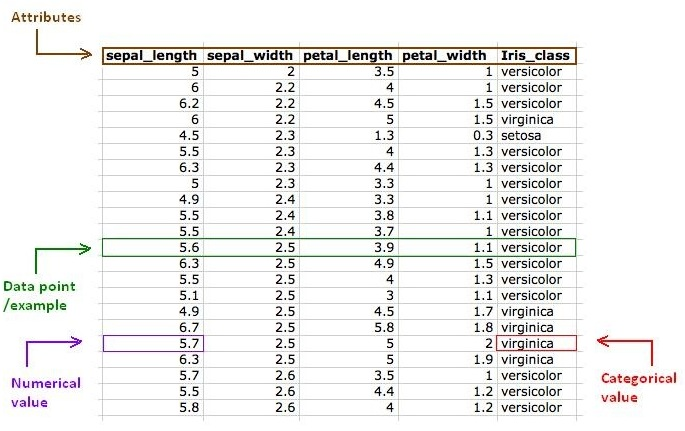
\includegraphics[width=13cm]{datasetIris.jpg}
\caption{Dataset iris}
\label{fig:iris}
\end{figure}
\\
\newpage
\large
\section*{Descrizione del K-Means}
\addcontentsline{toc}{section}{Cos'è il K-Means}
L'algoritmo K-means è un algoritmo di \textbf{clustering partizionale} che permette di suddividere un insieme di oggetti (punti) in K gruppi sulla base dei loro attributi, ossia raggruppare per oggetti "simili". \\
\begin{figure}[htp]
\centering
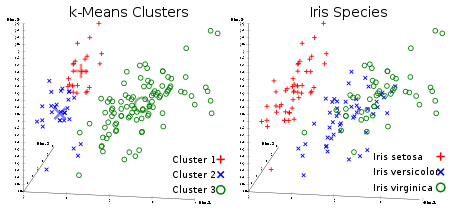
\includegraphics[width=16cm]{kMeans.png}
\caption{Visualizzazione del clustering mediante K-Means}
\label{fig:kmeans}
\end{figure}
\\
\subsection*{Algoritmo}
 \addcontentsline{toc}{subsection}{Algoritmo}
L'obiettivo che l'algoritmo si prepone è di minimizzare la varianza totale intra-cluster. Ogni cluster viene identificato mediante un \textbf{centroide} o punto medio. L'algoritmo segue una procedura iterativa: inizialmente crea K partizioni (K è l'unico valori di input) e assegna ad ogni partizione i punti d'ingresso o casualmente o usando alcune informazioni euristiche (conoscere a priori alcuni oggetti ed ecc) utilizzando la minima distanza euclidea (\textbf{MDM}).
\begin{figure}[htp]
\centering
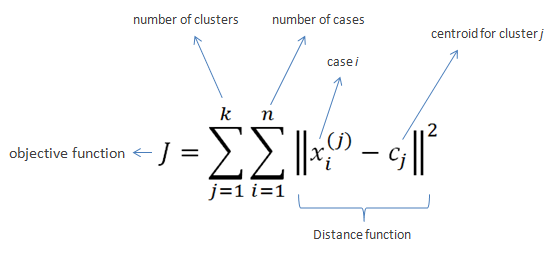
\includegraphics[width=7cm]{mdm.png}
\caption{Applicazione della distanza euclidea}
\label{fig:mdm}
\end{figure}
\\
Quindi calcola il centroide di ogni gruppo costruendo così una nuova partizione associando ogni punto d'ingresso al cluster il cui centroide è più vicino ad esso. Quindi vengono ricalcolati i centroidi per i nuovi cluster come la media dei punti calcolati per ogni cluster e così via, finché l'algoritmo non converge. \\
Attenzione: la convergenza \textbf{non è sempre garantita} scegliendo K cluster poichè potrebbero essere scelti dei centroidi così vicini, da creare meno gruppi di quelli che dovrebbero essere presenti.\\
\begin{figure}[htp]
\centering
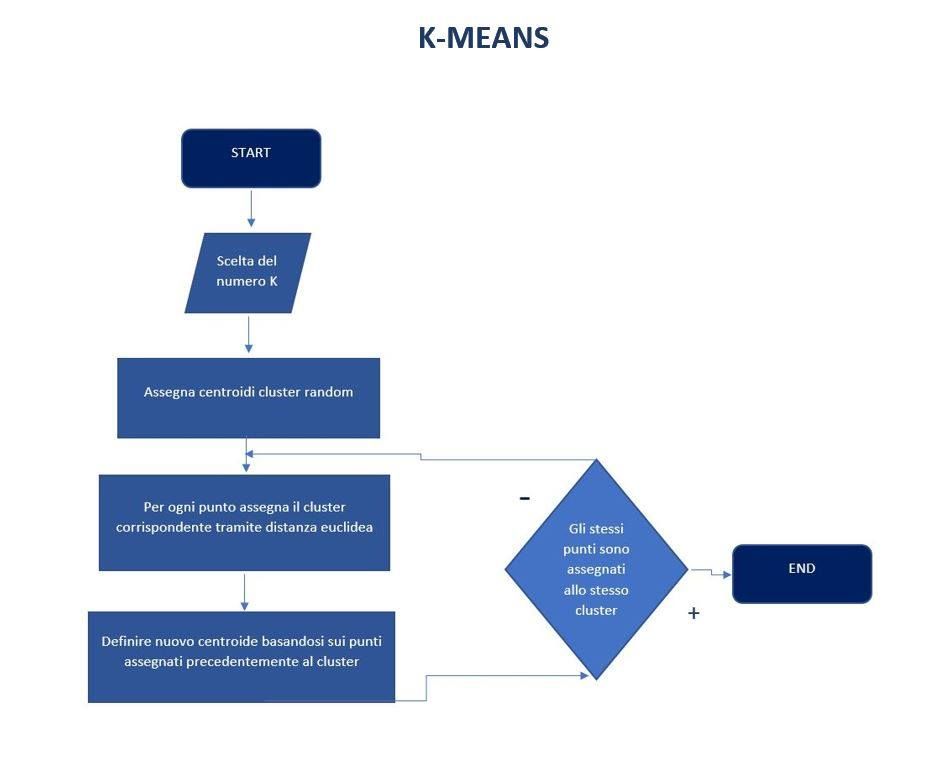
\includegraphics[width=17cm]{algoritmo.jpg}
\caption{Algoritmo seguito per la realizzazione del K-Means}
\label{fig:algoritmo}
\end{figure}

\newpage
\large
\section*{Analisi delle Componenti Principali (PCA)}
\addcontentsline{toc}{section}{Analisi delle Componenti Principali (PCA)}
L'analisi in componenti principali o PCA, dall'inglese principal component analysis, è una tecnica per la semplificazione dei dati utilizzata nell'ambito della statistica multivariata. \\
Lo scopo primario di questa tecnica è la riduzione di un numero più o meno elevato di variabili (rappresentanti altrettante caratteristiche del fenomeno analizzato) in alcune variabili latenti (feature reduction). Infatti tale è necessaria nel caso si volesse visualizzare un dataset con un numero di Features maggiori di 3, poichè non sarebbe possibile effettuare la visualizzazione, senza perderne il contenuto informativo. \\
Ciò avviene tramite una trasformazione lineare delle variabili che proietta quelle originarie in un nuovo sistema cartesiano nel quale la nuova variabile con la maggiore varianza viene proiettata sul primo asse, la variabile nuova, seconda per dimensione della varianza, sul secondo asse e così via. La riduzione della complessità avviene limitandosi ad analizzare le principali (per varianza) tra le nuove variabili. 
\\
\begin{figure}[htp]
\centering
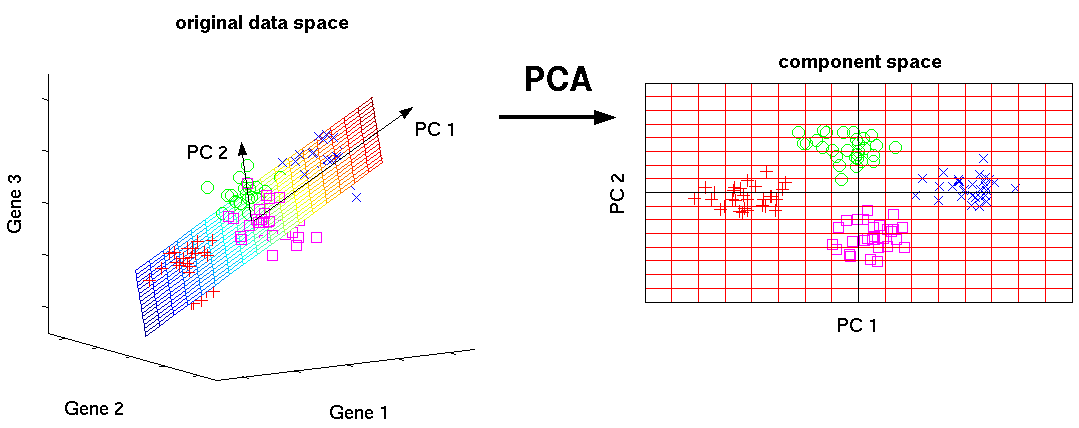
\includegraphics[width=14cm]{pca.png}
\caption{Realizzazione di una PCA}
\label{fig:pca}
\end{figure}
\\
Ciò avviene tramite una trasformazione lineare delle variabili che proietta quelle originarie in un nuovo sistema cartesiano nel quale la nuova variabile con la maggiore varianza viene proiettata sul primo asse, la variabile nuova, seconda per dimensione della varianza, sul secondo asse e così via.
La riduzione della complessità avviene limitandosi ad analizzare le principali (per varianza) tra le nuove variabili.





\pagestyle{myheadings} 
\markboth{\MakeUppercase{Progettazione}}{\MakeUppercase{Progettazione}}\chapter*{Progettazione}
\addcontentsline{toc}{chapter}{Progettazione}
\pagestyle{myheadings} 

\large



\section*{Analisi}
\addcontentsline{toc}{section}{Analisi}
Analizzando il problema si è deciso di sviluppare la progettazione di
un sistema, suddividendo la modellazione e sviluppo in due macro-parti:
\begin{itemize}
\item La prima che si occuperà del \textbf{BACK-END}, nello specifico di \textit{"forinire le strutture dati e le funzionalità necessarie alla creazione del Dataset e del Datamining"}. \\
Il \textit{Dataset} è caratterizzato dalle seguenti peculiarità:
     \begin{itemize}
        \item{\textbf{Informazioni fondamentali sul Dataset}, come il nome e il nome delle features (ad esempio Iris avrà lunghezza petalo, larghetta petalo ed ecc...);}
        \item{\textbf{Caricamento del dataset}, cioè descrizione dei passaggi per caricare un determinato dataset. Nel caso di iris sarà un caricamento di un file .data, ma in generale può cambiare per ogni specifico dataset;}
        \item{\textbf{Memorizzazione dai dati}, cioè come verranno memorizzati i record o osservazioni del dataset nella adeguata strutture dati che rappresenterà la tabella relazionale (o una matrice).}
      \end{itemize}

Il \textit{Data Mining} rappresenta un insieme di metodi e tecniche sintetizzati nel seguente modo: 
     \begin{itemize}
        \item{\textbf{Decisione del Dataset} su cui operare;}
        \item{\textbf{Selezione delle features}, cioè decidere quali caratteristiche o features scegliere per la clusterizzazione;}
        \item{\textbf{Clusterizzazione mediante l'algoritmo K-Means}, indicando il numero K di cluster.\\ NB la clusterizzazione non fornisce ancora la visualizzazione, perchè dipenderà dal gestore del front-end plottare i vari grafici.}
      \end{itemize}
\item La seconda parte si occuperà del \textbf{FRONT-END}, nel dettaglio nel \textit{"fornire un'adeguata GUI in JavaFX per una maggior esaltazione della user experience"}.
         \begin{itemize}
        \item{\textbf{Creazione di un menù} per garantire l'interazione con l'utente;}
        \item{\textbf{Applicazione di una grafica adeguata}, cioè mediante una serie di applicazione di fogli di stile e vari accorgimenti grafici;}
        \item{\textbf{Visualizzazione del risultato del clustering}, cioè la visualizzazione dei grafici 2D/3D utilizzati per l'output del DataMining.}
      \end{itemize}
\end{itemize} 
Entrambe le macro-parti, sono stati analizzate utilizzando il paradigma della \textbf{programmazione orientata agli oggetti (OOP)}, individuando le caratteristiche principali descritte sopra. \\
Il linguaggio utilizzato per la progettazione è \textbf{Java 8 SE} (utilizzando anche nuovi costrutti), mentre è stato utilizzato unicamente \textbf{JavaFX} (oramai standard di java) per l'interfaccia grafica.

\large
\section*{Novità di Java 8 utilizzate}
\addcontentsline{toc}{section}{Novità di Java 8 utilizzate: Espressioni Lambda}
\subsection*{Espressioni Lambda}
\addcontentsline{toc}{subsection}{Espressioni Lambda}
Come visto durante il corso, tra le varie novità di Java 8 sono presenti il potenziamento delle interfacce, integrando metodi statici (non vengono ereditati) e definendo i metodi di default che rappresentano dei metodi concreti che saranno ereditati, facendo attenzione al Diamond Problem.\\
Per la progettazione sono state utilizzate le \textbf{Espressioni LAMBDA} che rappresentano una sintassi più semplice e leggibile per definire-creare un'istanza di una classe anonima che implementa un'interfaccia con un solo metodo astratto (interfaccia funzionale). Si consideri la seguante equivalenza per capirne il funzionamento:\\

\lstset{language=Java,numbers=none, numberstyle=\scriptsize, frameround=fttt, breaklines=true, showstringspaces=false,
	 basicstyle=\scriptsize\ttfamily, keywordstyle=\color{blue}\bfseries, stringstyle=\color{red}, commentstyle=\color{green}}
%esempio codice Java	 
\begin{lstlisting}
lambda-parametri -> lambda-corpo
\end{lstlisting}

Si noti lo speciale segno "->". Questa è praticamente equivalente a:
\begin{lstlisting}
new NomeI() {
    metodo(lambda-parametri) {
        lambda-corpo
    }
}
\end{lstlisting}
Nel progetto si è fatto un largo uso, ad esempio per registrare l'evento di evidenziare la colonna di una corrispondente checkbox:
\begin{lstlisting}
/* Verifica se tale colonna dovrà essere selezionando controllando la corrispondente checkbox se è selezionata.*/
boxes[i].selectedProperty().addListener(/* Lambda expression con changeListener e changer */
	(obs, wasSelected, isNowSelected) -> //parametri disponibili per override
	{
	/* Se il box è stato selezionato aggiungilo tra le colonne da evidenziare, altrimenti toglielo da quelle evidenziate. */
            if (isNowSelected) {
                highlightColumns.add(col);
            } else {
                highlightColumns.remove(col);
            }
     });
\end{lstlisting}
In generale può essere utilizzata anche per riferimento a metodo o a costruttori mediante il simbolo '::'che non sono anonime, ma che si riferiscono ad un specifico metodo di una determinata classe (o di una istanza). Di seguito un esempio completo:
\begin{lstlisting}
//Senza Lambda
List list1 = Arrays.asList(1,2,3,5);
for(Integer n: list1) {
    System.out.println(n);
}
/*foreach è metodo che accetta consumer, un'interfaccia funzionale che corrisponde all'azione da eguire per ogni elemento della lista*/
//Lambda Anonime 
List list2 = Arrays.asList(1,2,3,5);
list2.forEach(n -> System.out.println(n)); 
//Lambda con Riferimenti anonimi, 
list2.forEach(System.out::println);
\end{lstlisting}

\large
\subsection*{JavaFX}
\addcontentsline{toc}{subsection}{JavaFX}
JavaFX è una famiglia di software applicativi (\textbf{Framework}) divenuti ormai standard di Java8 SE, utilizzata soprattutto per la creazione di applicazioni web che hanno tutte le caratteristiche e funzionalità delle comuni applicazioni per computer. Con JavaFX è possibile realizzare delle applicazioni per computer, cellulari (andoroid o iOS), dispositivi portatili di vario genere, televisori e altri tipi di piattaforme.\\ \\
Lo spazio grafico di lavoro di JavaFX è un oggetto \textbf{Stage}, radice di ogni applicazione JavaFX 8 (finestra), che può contenere uno o piu oggetti \textbf{Scene}, che a loro volta contengono generici componenti grafici (\textbf{Node}) che presentano delle proprie proprietà (\textit{Property}). Il concetto ricorda molto quello di DOM di una pagina HTML, in cui possono essere disposti opportuni tag con alcuni attributi.
\\
\begin{figure}[htp]
\centering
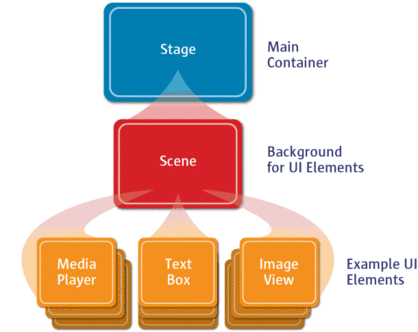
\includegraphics[width=8cm]{stage.png}
\caption{Idea dell'albero utilizzato da JavaFX}
\label{fig:JavaFX}
\end{figure}
\\
Java FX organizza la grafica un'insieme di nodi organizzati in una struttura ad albero, mediante un formato di Markup \textbf{FXML}, derivante da XML, che fornisce la struttura di un'interfaccia grafica separandola dal codice dell'applicazione consentendo di assemblare interfacce grafiche senza utilizzare codice Java. FXML non è un linguaggio compilatoe quindi non necessita di compilazione. Utilizzando il pattern \textbf{MVC} e un controller, diventa molto semplice la manipolazione.
\\
Ricapitolando, queste sono le principali peculiarità che rendono molto interessante JavaFX:
     \begin{itemize}
        \item{Immediato uso del \textbf{pattern Architetturale MVC};}
        \item{Supporta il formato e i file \textbf{CSS}, ossia fogli di stile utilizzati per dare maggior enfasi grafica;}
        \item{Supporto a motore grafico 2D/3D;}
        \item{Integrazione di grafici scientifici;}
        \item{Portabilità e multipiattaforma;}
        \item{Facile costruzione di Layout Statici e Dinamici;}
      \end{itemize}
File .FXML, .CSS e utilizzo delle routine principali di JavaFX sono presenti nel progetto.



\newpage
\large
\section*{Organizzazione e struttura progetto}
\addcontentsline{toc}{section}{Organizzazione e struttura progetto}
La progettazione delle classi e la costruzione dell'applicazione è avvenuta utilizzando l'idee \textit{"Eclipse Java EE IDE Versione: Mars.1 (4.5.1)"}.\\
Le principali librerie da linkare utilizzate per la progettazione sono:
     \begin{itemize}
        \item{\textbf{JavaFX SDK;} per utilizzare javafx}
        \item{\textbf{colt-1.2.0.jar}, sviluppata dal CERN (Organizzazione europea per la ricerca nucleare) necessaria per la costruzione della classe 'PCAcolt', indispensabile per applicare la PCA.}
      \end{itemize}

\\
\begin{figure}[htp]
\centering
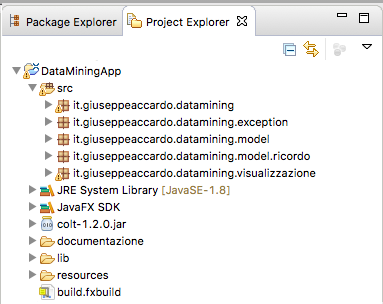
\includegraphics[width=13cm]{struttura.png}
\caption{Struttura del progetto in Eclipse}
\label{fig:Struttura elcipse}
\end{figure}

\\
Si può osservare che il primo package è quello contenente i file principali dell'applicazione. Tali apparterranno, come si vedrà successivamente, alla \textbf{'View'} e \textbf{'Controller'} utilizzati per visualizzare il menu, gestire le interazioni con esso e visualizzare il grafico (grazie all'uso delle classi all'interno dell'ultimo package).\\
Il secondo package è utilizzato per contenere particolare eccezioni utilizzare dal controller per la visualizzazione di alert o conferme.\\
I package che terminano con 'model' e 'model.ricordo' sono invece i \textbf{'Model'} utilizzati dal controller per il funzionamento dell'intera applicazione.
\\ 
Inoltre sono presenti cartelle per la documentazione (JavaDOC) e rouserces per vari file (file dataset e immagini).
\\
Il progetto presenta applicazioni di 'Ingegneria del Software' mediante l'utilizzo di Design Pattern per la risoluzione di varie problematiche più complesse. Infatti permettono di ottenere delle soluzioni, seguendo degli "schemi" o "pattern" che a priori permettono di risolvere i problemi.\\
\newpage
In totale ne sono stati utilizzati 6 e sono i seguenti:
     \begin{itemize}
        \item{\textbf{MVC}}
        \item{\textbf{Strategy}}
        \item{\textbf{Template Method}}
        \item{\textbf{Observer}}
                \item{\textbf{Memento}}
                        \item{\textbf{Prototype}}
      \end{itemize}
Più avanti ne approfondiremo l'applicazione.


\newpage
\section*{MVC}
\addcontentsline{toc}{section}{MVC}
Il Model-View-Controller (MVC) è un \textbf{Pattern Architetturale} molto diffuso nello sviluppo di sistemi software (applicazioni J2EE, .NET ed ecc), in particolare nell'ambito della programmazione orientata agli oggetti, in grado di separare la logica di presentazione dei dati dalla logica di business. 
\\
Tale pattern è composto da 3 componenti che comunicano tra loro e sono:
     \begin{itemize}
        \item{\textbf{Model};}
        \item{\textbf{Controller};}
        \item{\textbf{View}.}
      \end{itemize}
\begin{figure}[htp]
\centering
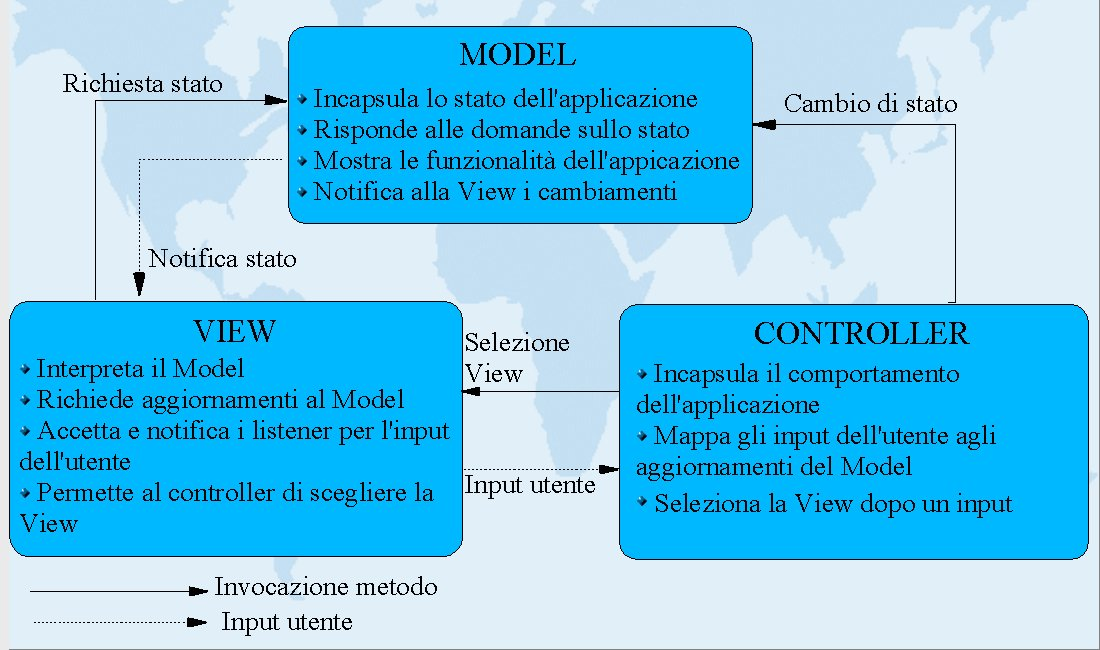
\includegraphics[width=14cm]{mvc.jpg}
\caption{Tipico funzionamento dell'MVC}
\label{fig:mvc}
\end{figure}
\\
In questa applicazione il \textbf{Model} è realizzato mediante le classi 'Dataset' e 'Datamining' poichè forniscono l'entry per accedere ai dati e di memorizzarne uno stato in base alle richieste del client. Quindi il funzionamento del DataMining e del K-Means è completamente trasparente all'utente, cioè si dice che sia a livello \textit{Back-End}. \\ Il model rappresenta l'insieme delle classi all'interno dei package  \textit{it.giuseppeaccardo.datamining.model} e \textit{it.giuseppeaccardo.datamining.model.ricordo}.\\
\\
Il \textbf{Controller} ha il compito di ricevere i comandi dall'utente (attraverso la \textbf{GUI} appartenente view) e di mapparne tutti gli aggiornamenti e cambiamenti di stato verso il model. Effettuate tale modifiche, il controller selezionerà la view su cui voler mostrare i gli eventuali risultati del model o effettuare una determinata azione (rendere il layout dinamico).\\
Il controller è realizzato mediante la classe \textit{DataminingController.java} contenuta nel package principale \textit{it.giuseppeaccardo.datamining}. Da notare che l'MVC effettua una divisione comportamentale e logica delle componenti, quindi ad esempio parte di View sarà contenuta anche nel controller.
\\
\\
La \textbf{View} si occupa di interpretare il model a livello di \textit{Front-end} (interfaccia utente grafica o GUI). Da esso possono partire delle richieste verso il controller che risponderà, ma può richiedere anche semplicemente lo stato direttamente al model o ricevere da esso una notifica di cambiamento di stato. \\Questo legame (in ambito di JavaFX è detto \textbf{Binding}) è effettuato mediante il design pattern \textit{\textbf{"Observer"}}  per definire un forte dipendenza tra view e model in modo tale che se una cambia, l'altra è aggiornata automaticamente. \\In JavaFX tale design pattern è implementato direttamente mediante la collection interface \textbf{'ObservableList<E>'} che appunto tiene traccia di tutti i dati e dei suoi aggiornamenti.\\
Nel progetto la view è rappresentato dal layout sviluppato in \textbf{FXML}, comprendenti di fogli di stie \textbf{CSS} e dal \textbf{Main} che si occupa di lanciare lo stage su cui andranno le scene da far visualizzare all'utente. Tali moduli sono presenti sempre in \textit{it.giuseppeaccardo.datamining}, appunto per le forti correlazioni che si hanno tra view e controller. Inoltre anche \textit{it.giuseppeaccardo.datamining.visualizzazione} e \textit{it.giuseppeaccardo.datamining.exception} vengono utilizzate dal controller per fornire alla view grafici o alert di attenzione (eccezioni).\\
\\
Come detto la scelta di costruire l'applicazione solo con JavaFX è perchè presenta una serie di vantaggi (costruzioni di grafici, facile comunicazione con altri software ed ecc..), ma soprattutto perchè è già predisposto per la costruzioni di applicazioni seguendo il Design Pattern MVC. Infatti, come detto prima, fornisce già strutture che facilitano il compito di determinate operazioni, come l'aggiornamento dei dati che è direttamente implementato mediante l'ObservableList che presenta le funzionalità dell'Observer pattern. \\
Inoltre l'MVC garantisce una facile portabilità di sistema (Servlet ed ecc).

\newpage
\large
\section*{Principi SOLID}
\addcontentsline{toc}{section}{Principi SOLID}
I principi \textbf{SOLID} sono stati introdotti da Robert C. Martin, uno dei padri delle metodologie agili, consentendo di avere un software estendibile e manutenibile, evitando di avere software rigido, difficile da cambiare, con cut and paste inutili e complesso \textbf{(code smells)}. L'acronimo corrisponde ai seguenti principi:

      \begin{itemize}
      
         \item \textbf{Single Responsability Principle (SRP) }

        \item \textbf{Open Closed Principle (OCP)}


        \item \textbf{Liskov's Substitution Principle (LSP)}


        \item \textbf{Interface Segregation Principle (ISP)}
        

        \item \textbf{Dependency Inversione Principle (DIP)}

      \end{itemize}
    

Nello specifico tecnico:\\
   \begin{enumerate}
      
         \item \textbf{Single Responsability Principle (SRP) }\\
Una classe dovrebbe avere un solo motivo per cambiare ogni elemento di un programma (classe, metodo, variabile) deve avere una sola responsabilit`a tale responsabilità debba essere interamente incapsulata dall'elemento stesso. Questo principio afferma che se una classe può cambiare per 2 motivi allora dobbiamo dividere le responsabilità in 2 classi, ogni classe gestisce solo una responsabilita`. Si consideri un modulo che compila e stampa un report, tale modulo puà cambiare per due motivi: il contenuto del report oppure il formato del report, questi due aspetti sono due responsabilita` distinte e vanno descritte in classi o moduli separati. Sarebbe cattiva progettazione accoppiare due cose che cambiano per motivi diversi in momenti diversi.

        \item \textbf{Open Closed Principle (OCP)}\\
Le entità software come classi, moduli e funzioni dovrebbero essere aperte per l'estensione, ma chiuse per le modifiche. Il principio stabilisce che la progettazione del software deve essere fatta in modo che le nuove funzionalita` sono aggiunte con il minimo cambiamento possibile nel codice esistente. Quando scriviamo una classe dobbiamo garantire che per una sua estensione non c'`e bisogno di cambiare la classe stessa. Casi particolari di OCP: Template pattern, Strategy pattern, anche i pattern Decorator, Factory Method, Observer ci aiutano a rispettare OCP.
        \item \textbf{Liskov's Substitution Principle (LSP)}\\
I tipi derivati devono essere completamente sostituibili ai loro tipi base. Dobbiamo essere sicuri che nuove classi derivate stanno estendendo le loro classi base senza cambiare il comportamento. Le classi derivate dovrebbero essere capaci di rimpiazzare le classi base senza cambiamenti nel codice, altrimenti le nuove classi producono e↵etti indesiderati sul funzionamento del programma. Questo è un'estensione di OCP.
        \item \textbf{Interface Segregation Principle (ISP)}\\
Un client non dovrebbe dipendere da metodi che non usa. E` preferibile che le interfacce sia molte, specifiche e piccole (composte da pochi metodi) piuttosto che poche, generali e grandi. Quando progettiamo software dobbiamo stare attenti a come definiamo le interfacce, se contengono molti metodi puo` capitare che vengono utilizzate da un modulo che contiene solo alcune di quelle funzionalita`, siamo obbligati a implementare l'interfaccia completa e ritrovarci con metodi inutilizzabili.
        \item \textbf{Dependency Inversione Principle (DIP)}\\
I moduli di alto livello non dovrebbero dipendere dai moduli di basso livello. Entrambi dovrebbero dipendere dalle astrazioni. Le astrazioni non dovrebbero dipendere dai dettagli. I dettagli dovrebbero dipendere dalle astrazioni. In un cattivo sviluppo del software le classi ad alto livello dipendono pesantemente da quelle a piu` basso livello. Quando progettiamo un software definiamo classi di basso livello quelle che implementano le operazioni di base (accesso al disco, protocollo di rete ecc.)be classi di alto livello quelle che incapsulano la logica di business, un approccio naturale di sviluppo `e quello di scrivere prima le classi di basso livello e poi quello di alto livello, ma questo non `e un modo di progettare flessibile: nel caso in cui dobbiamo sostituire una classe di basso livello abbiamo che le classi di alto livellodipendono pesantemente da quelle di basso livello e questo comporta la modifica anche nelle classi di alto livello. Per evitare questo tipo di problemi possiamo introdurre uno strato intermedio (astrazione) tra le classi di alto livello e quelle di basso livello: le classi di alto livello non devono dipendere da quelle di basso livello lo strato intermedio non deve essere creato basandosi su le classi di basso livello, le classi di livello basso sono create basandosi sullo strato intermedio.
\end{enumerate}


Il progetto è stato sviluppato ponendo attenzione al rispetto dei principi SOLID riporto un esempio per ognuno dei principi:
    \begin{enumerate}
      
         \item \textbf{Single Responsability Principle (SRP) }\\
         Ogni singola classe è costruita in modo tale da avere classi con singole riesponsabilitò.\\
         Ad esempio visualizzazione grafica è una classe separata rispetto dalla classe Datamining. Infatti in base al contenuto di un Datamining, viene generato in un apposita classe una nuova classe Visualizzazione che presenta delle responsabilità distinte. 
        \item \textbf{Open Closed Principle (OCP)}\\
         Le classi sono molto più predisposte all'estensione, che alla modifiche delle stesse.\\ Come detto in precedenza, utilizzando classi astratte o determinati pattern, come il Template o lo Strategy, riusciamo a garantire facilmente questo principio. Un ottimo esempio è il Template utilizzato per fornire un Framework di Dataset, in cui il Dataset concreto (come Iris) non necessita di effettuare cambiamenti alla classe stessa, poichè è aperta all'estensione. Stessa considerazione vale per Visualizzazione poichè utilizza lo Strategy Pattern.
        \item \textbf{Liskov's Substitution Principle (LSP)}\\
        Il principio di Liskov è ampiamente garantito. \\Basta osservare che le implementazioni concrete di Visualizzazione o Dataset, potrebbero essere completamente sostituite dal altri tipi derivati, senza perderne la logica. Questo è garantito, oltre dai pattern applicati, dall'uso di interfacce e classi astratte. Il principio non è applicato in modo "severo". Teoricamente, anche ArrayList<E> dovrebbe essere dichiarato come un List<E> poichè è la collection da cui estende.

        \item \textbf{Interface Segregation Principle (ISP)}\\
        Tale principio è soddisfatto poichè vengono utilizzate un numero consistente di interfacce che presentano pochi metodi.\\ In particolare non sono presenti casi in cui è stato dovuto applicare (ad esempio un'interfaccia con tanti metodi scissa in più interfacce).
        
        \item \textbf{Dependency Inversione Principle (DIP)}\\
        I moduli di alto livello non dipendono da quelli di basso livello, mentre i dettagli si.\\
        Il caricamento del dataset viene effettuato da una sua implementazione concreta (Iris in questo caso) che ne implementa un comportamento a basso livello, mentre dataset fornisce presenta giusto la logica da seguire. Un ottimo pattern da utilizzare sarebbe stato il DAO, non approfondito nel corso.
    \end{enumerate}

 \newpage
 \section*{Diagrammi UML}
\addcontentsline{toc}{section}{Diagrammi UML}
Questo è il diagramma UML completo delle 21 classi dell'intero sistema di JavaFX, contenente le componenti MVC.
\\ Le classi sono rigorosamente commentate e spiegate in modo dettagliato nella documentazione del JavaDOC.\\

 \begin{figure}[htp]
\centering
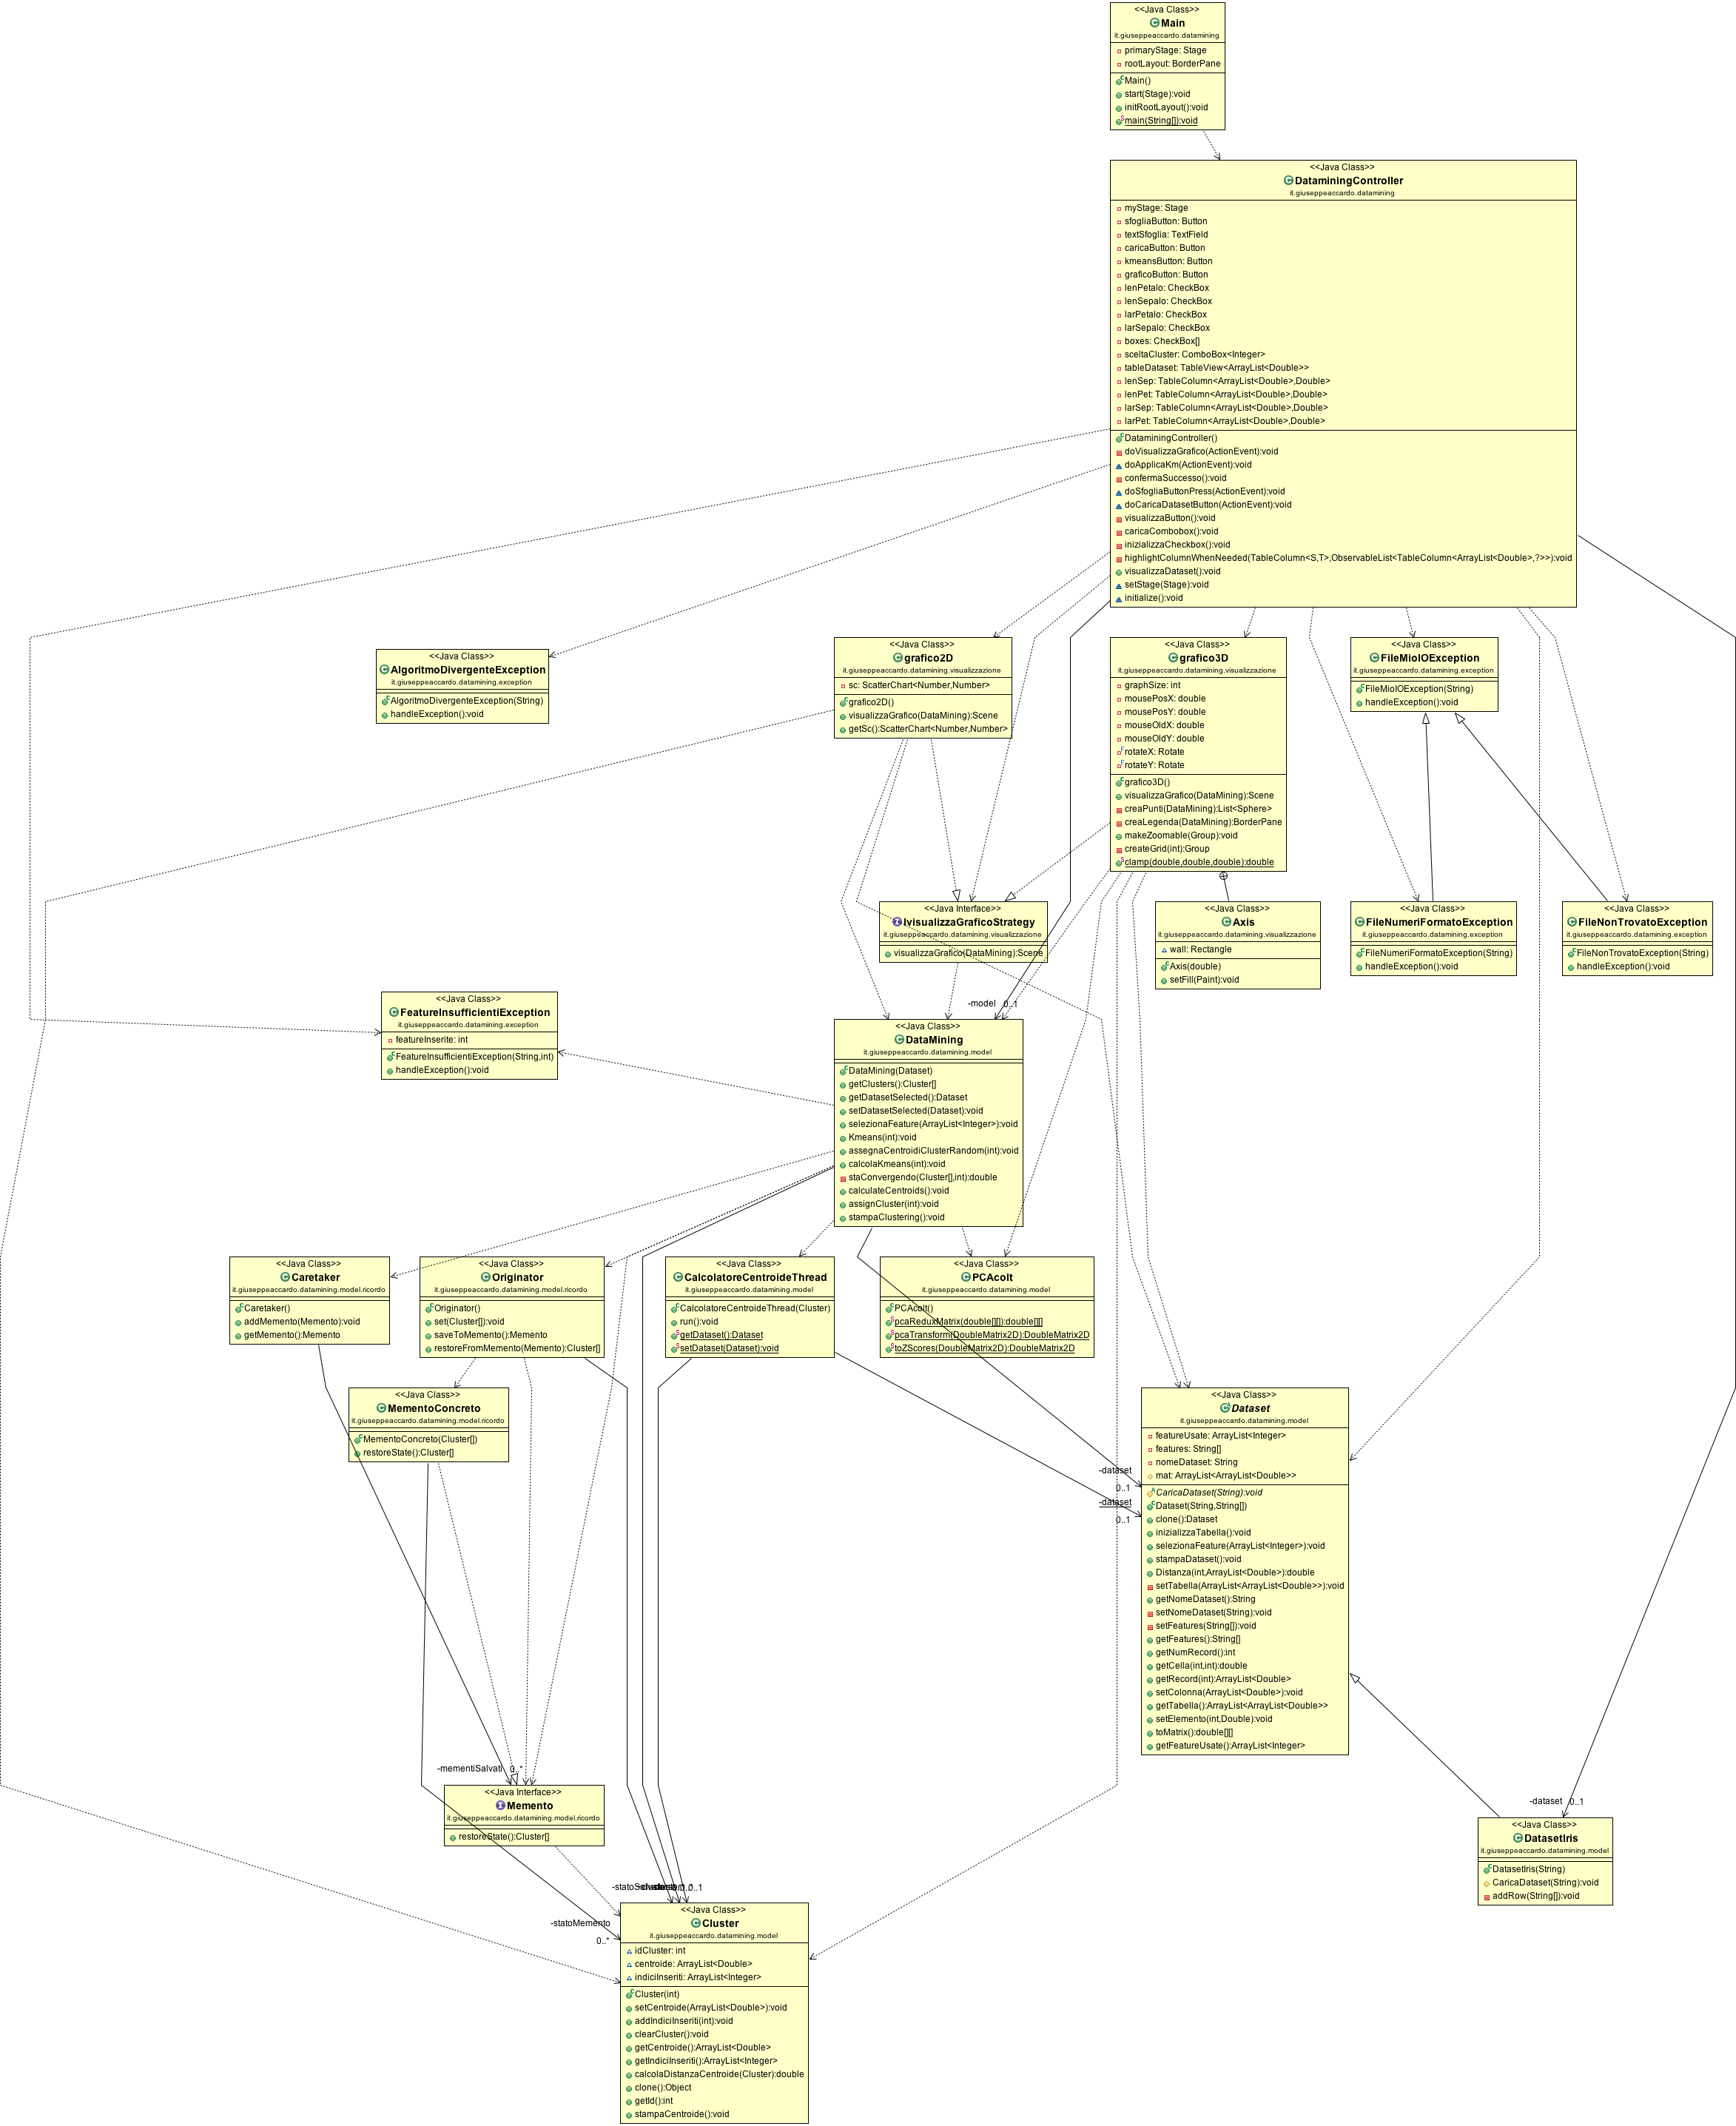
\includegraphics[width=14cm]{umlCompleto.png}
\caption{UML completo di tutte le classi utilizzate}
\label{fig:uml completo}
\end{figure}

 \newpage
Suddividendo le classi per package:
\begin{itemize}

 \item \textit{\textbf{it.giuseppeaccardo.datamining}}\\
 Package contenente l'insieme dei file necessari per il funzionamento di JavaFX.\\
 \textbf{Main} è la classe principale dell'applicazione in JavaFX. Esso rappresenta la parte "View" che si occupa di impostare un "Layout" predefinito in formato FXML, ossia la parte statica dell'applicazione, con l'opportuno foglio di stile CSS. Main estende application e il metodo che eredita più importante è il metodo start(Stage primaryStage). Questo è automaticamente chiamato quando l'applicazione viene lanciata dall'interno del metodo main. Lo stage indica la finestra su cui agganciare le scene che a loro volta conterranno la disposizione degli oggetti grafici (per definire la GUI).\\
 Il layout da cui caricare l'interfaccia è il file FXML \textit{Datamining.fxml}  (formato di javaFX non compilato), mentre lo stile CSS è caricato dal file \textit{application.css}.\\
 
Ad un file FXML  associato un controllore, rappresentato dallla classe \textbf{dataminingController}, che è una classe java che gestisce gli elementi grafici ad esempio impostando l'azione richiesta quando si preme un pulsante. Quindi è il pilastro dell'interazione e della user-interface dell'utente.\\
Per gestire aggiornamenti tra View-Controller e notifiche di stato, viene utilizzata la collection \textit{\textbf{ObservableList<E>}} che auto-implementa il design pattern \textbf{Observer}.
 \begin{figure}[htp]
\centering
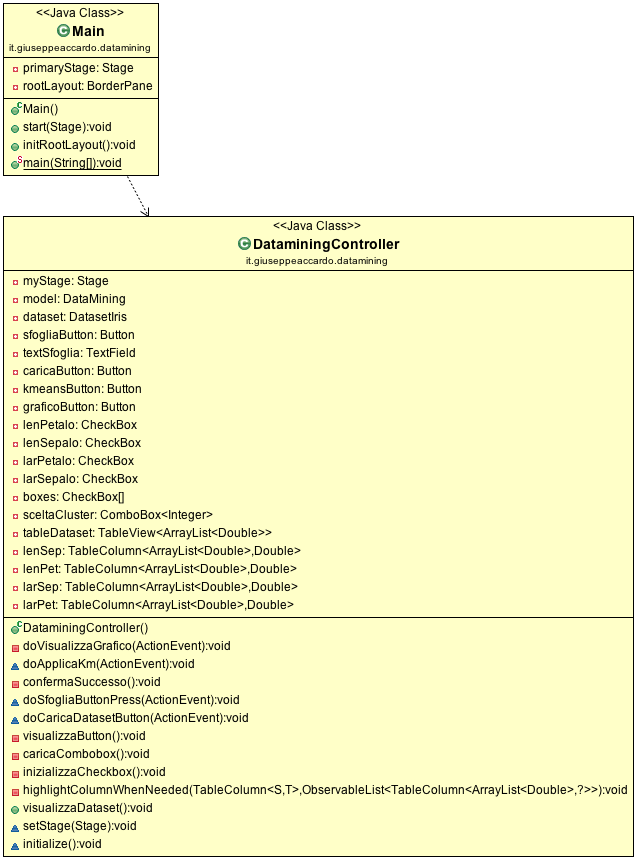
\includegraphics[width=9cm]{umlDataminingFX.png}
\caption{UML delle classi principali per gestire javaFX}
\label{fig:uml javaFX}
\end{figure}



 \item \textit{\textbf{it.giuseppeaccardo.datamining.exception}}\\
 Questo package contiene tutte le eccezioni create ed utilizzate per gestire degli eventi anomali. \\
 Eccezioni sono spiegate nel dettaglio nella documentazione, ma in generale vengono utilizzate per gestire la divergenza del K-Means, la scelta giusta delle features (minimo due), l'esistenza e formattazione giusta del file. \\
 NB tutte le eccezioni hanno come super padre la classe \textbf{Exception}
  \begin{figure}[htp]
\centering
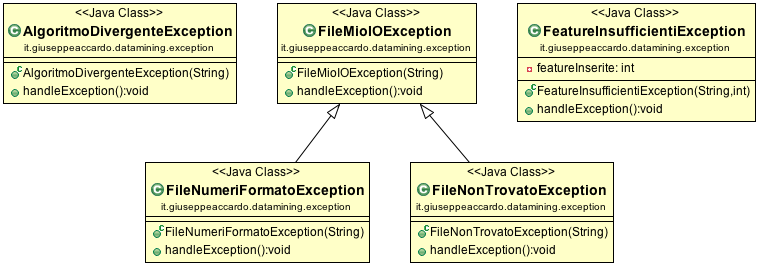
\includegraphics[width=14cm]{umlException.png}
\caption{UML delle classi per gestire le eccezioni}
\label{fig:uml eccezioni}
\end{figure}

 \item \textit{\textbf{it.giuseppeaccardo.datamining.model}}\\
Questo package contiene il Model.\\ 
\textbf{Dataset} è una classe astratta (CaricaDataset è un metodo astratto) utilizzata fondamentalmente per realizzare uno 'Scheletro' iniziale di un dataset. Il dataset costituisce un insieme di dati strutturati in forma relazionale, cioè corrisponde al contenuto di una singola tabella sottoforma di una matrice, dove le righe rappresentano i 'record' e le colonne le 'variabili' dette 'features'. Tale classe è posta in tal modo poichè si vuole rinviare la responsabilità di "come caricare un dataset reale" alla classe che estende dataset, utilizzando la stessa struttura di dataset. Il principio seguito è quello del design pattern \textit{\textbf{Template Method}} che definisce lo scheletro di un algoritmo in un'operazione, rinviando alcuni passi alle sottoclassi client, cioè consente alle sottoclassi di ridefinire alcuni passi senza cambiare la struttura dell'algoritmo. Altri design pattern che potevano essere realizzati erano il "Factory Method" o "Decorator". Da notare che tale classe utilizza anche il design pattern \textit{\textbf{Prototype}}, mediante l'implementazione dell'interfaccia di 'Cloneable' (override di clone). Questo perchè quando si selezionano le features di un dataset, si ha la necessita di creare nuovi oggetti copiando il dataset non selezionato di partenza in tal modo da non perdere lo stato iniziale. Copiato il dataset, si selezioneranno solo le features richieste. \\
\textbf{Dataset Iris} è l'implementazione concreta di Dataset, in cui il metodo astratto "caricaDataset" (Template Method) viene ridefinito. \\
\textbf{Cluster} rappresenta il "grappolo" o gruppo, in cui sono agglomerati i punti del dataset "piu simili". Un cluster è rappresentato da un centroide e dall'indice del record della tabella. Da notare che il "Prototype" è utile anche in questo caso poichè si ha la necessità di clonare un cluster in un determinato stato.\\
\textbf{CalcolatoreCentroideThread} è necessaria per l'esecuzione dei thread in parallelo. Tale implementa l'interfacca Runnable di cui si riscrive il metodo run(), necessario per il thread poichè saranno inserite le operazioni che tale dovrà eseguire. In questo caso, i thread in parallelo, riceveranno un cluster su cui effettaure il calcolo del centroide utilizzando la media aritmetica e tenendo conto di quanti e quali elementi sono inseriti per ogni cluster.\\
La classe \textbf{DataMining} rappresenta l'insieme di tecniche e metodologie che hanno per oggetto l'estrazione di un sapere o di una conoscenza a partire da grandi quantità di dati e l'utilizzo scientifico, industriale o operativo di questo sapere. Le fasi principali del sistema sviluppate sono: selezione delle caratteristiche, clustering e visualizzazione. 
La selezione delle caratteristiche (features) prevede quali e quante features vogliamo analizzare del dataset. Datamining può effettuare una scrittura da console utilizzando \textit{PCAcolt}, classe utilizzata per effettuare l'Analisi delle Componenti principali. \\
Nella fase di clustering viene usato un algoritmo per “agglomerare” dati simile, ossia il \textit{K-Means} che prenderà in input il numero di cluster K su cui operare. La visualizzazione di tale operato è eseguita dalle classi presenti nel package "Visualizzazione", anche se tale classe può effettuare una visualizzazione semplice da console, e la memorizzazione dello stato dei cluster precedenti avviene mediante il design pattern \textit{\textbf{Memento}}, implementato nel package \textit{it.giuseppeaccardo.datamining.model.ricordo}.

  \begin{figure}[htp]
\centering
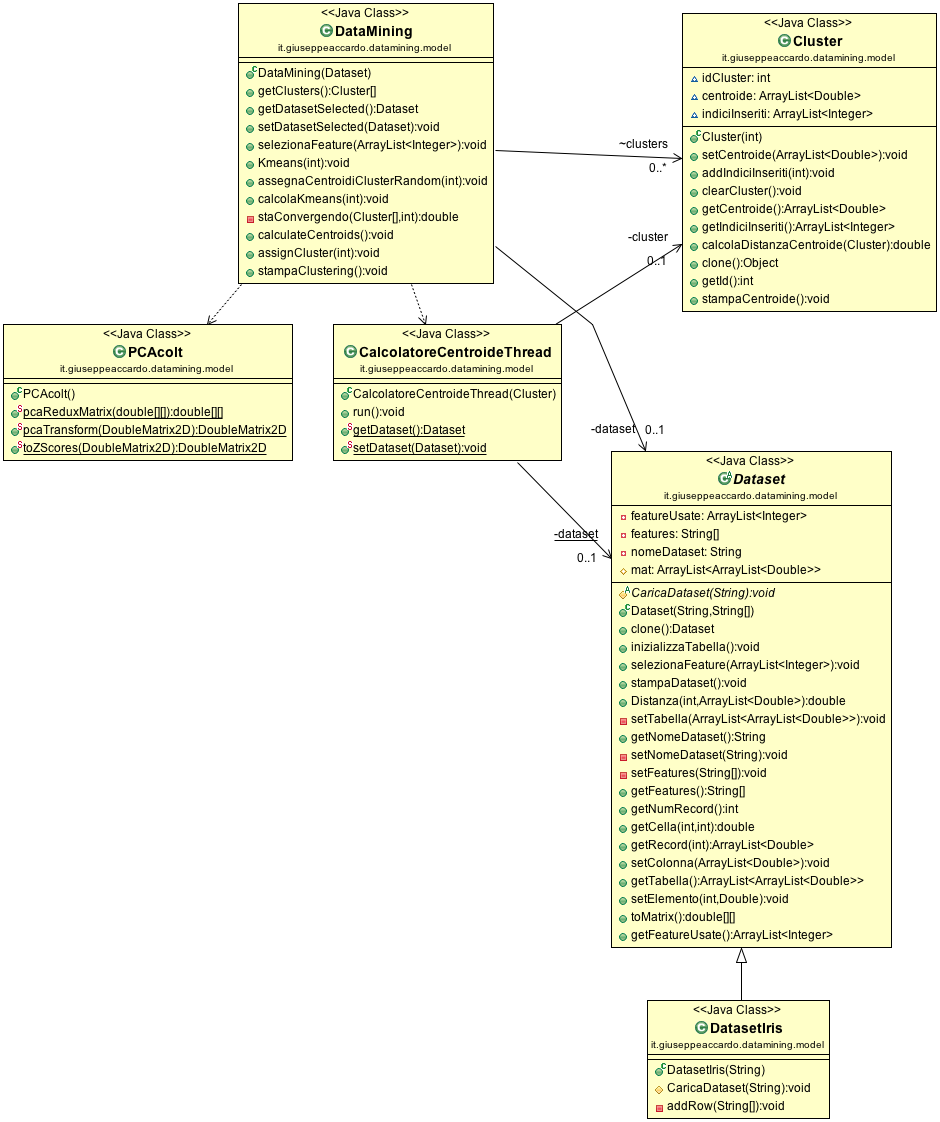
\includegraphics[width=12cm]{umlModel.png}
\caption{UML delle classi appartenenti al Model}
\label{fig:uml model}
\end{figure}


  \item \textit{\textbf{it.giuseppeaccardo.datamining.model.ricordo}}\\
  In questo package sono presenti le componenti fondamentale per l'utilizzo del design pattern \textit{\textbf{Memento}}. \\
  \\
  \textbf{Memento} rappresenta l'interfaccia che il  \textbf{ConcreteMemento} debba implementare per salvare un memento, cioè per immagazzinare lo stato generato da \textbf{Originator}. Quest'ultimo rappresenta l'istanza grazie alla quale viene generato uno stato fisico da salvare in Memento. \\Le istanze di ConcreteMemento saranno conservate in \textbf{Caretaker}.
  
  \begin{figure}[htp]
\centering
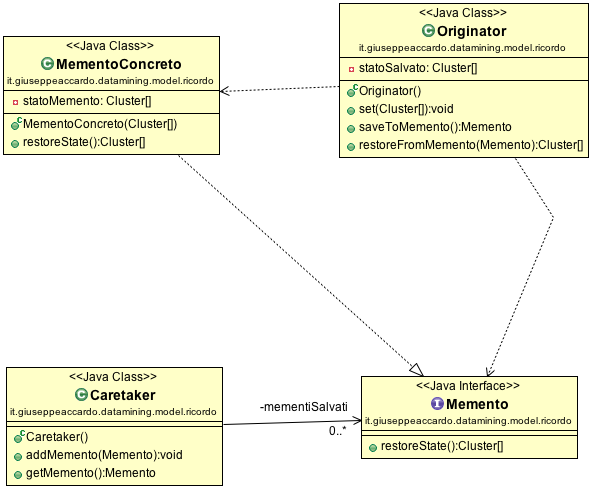
\includegraphics[width=13cm]{umlModelRicordo.png}
\caption{UML delle classi appartenenti all'implementazione di memento}
\label{fig:uml memento}
\end{figure}


 \item \textit{\textbf{it.giuseppeaccardo.datamining.visualizzazione}} \\
  Nel seguente package sono contenute le classi necessarie utilizzate da \textit{DataminingController} per creare le View che rappresenteranno i grafici 2D/3D della clusterizzazione.\\
  I Grafici 2D sono stati realizzati mediante le classi \textit{Chart} offerte da JavaFX, mentre i grafici 3D sono stati realizzati utilizzando il motore grafico tridimensionale fornito sempre da JavaFX, mediante la classe \textit{Shape3D}.\\
  Per craere un'intercambiabilità di grafici, ossia la necessità di modificare dinamicamente gli algoritmi, è stato applicato il design pattern \textit{\textbf{Strategy}}.\\
  Questa realizzazione avviene mediante l'interfaccia funzionale \textbf{IVisualizzaGraficoStrategy} che viene implementata sia da 
  \textbf{grafico2D} che da \textbf{grafico3D}. In modo tale, utilizzando come reference tale interfaccia, il metodo \textit{visualizzaGrafico} sarà 'virtuale', ossia a run time assumerà l'implementazione dell'oggetto corrispondente istanziato. Ad esempio, istanziando grafico2D, il metodo che sarà realmente invocato a run time sarà quello appartenente a grafico2D.\\
  Da notare che grafico3D utilizza la classe Axis per il disegno degli assi e PCAcolt per effettuare l'analisi delle componenti principali nel caso di features maggiori di 3.
  \\
  Il package, oltre a contenere le classi, contiene anche i file \textit{grafico2D} e \textit{grafico3D}  per la definizione dello stile dei grafici.\\
  
    \begin{figure}[htp]
\centering
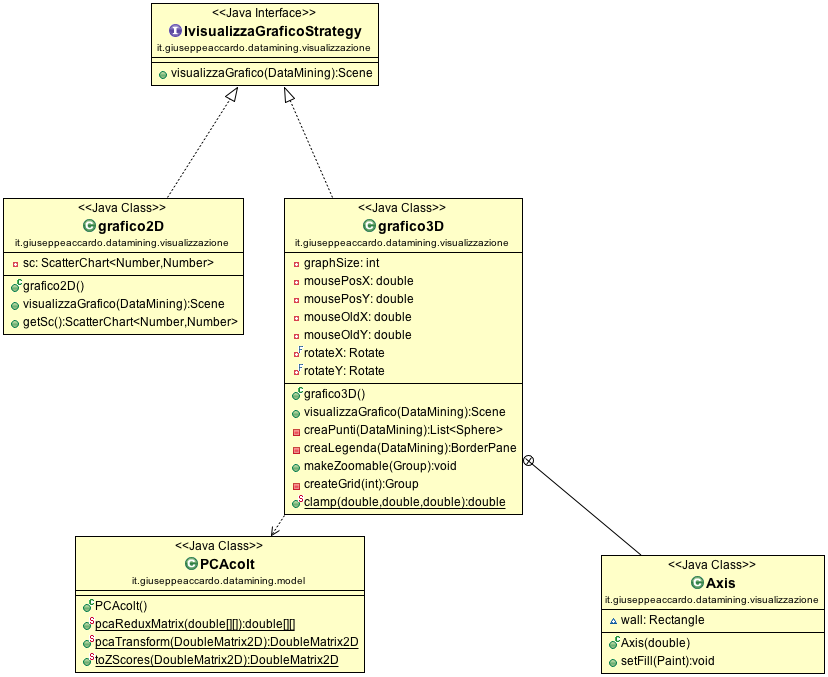
\includegraphics[width=13cm]{umlVisualizzazione.png}
\caption{UML delle classi appartenenti all'implementazione dello Strategy}
\label{fig:uml visualizzazione}
\end{figure}
\end{itemize}

 
 
\newpage

 
 
 \section*{Design Pattern}
\addcontentsline{toc}{section}{Design Pattern}
Il Design Pattern è un concetto che puo` essere definito come una soluzione progettuale generale ad un problema ricorrente. 23 Design Patterns sono stati raccolti e formalizzati concettualmente nel 1994 nel libro Design Patterns: Elements of Reusable Object-Oriented Software scritto da 4 autori successivamente noti come \textbf{Gang of Four (GoF)}.\\ 
l'utilizzo dei Pattern Designs comporta numerosi benefici:
\begin{itemize}
\item Forniscono un approccio industriale standard per risolvere un problema ricorrente consentendo di risparmiare tempo.
\item  Agevolano il riutilizzo di codice robusto e facile manutenere.
\item  L'utilizzo dei Design Patterns rende il codice facile da capire e da debuggare agli sviluppatori permettendo a nuovi membri del team di sviluppo di capire il codice piu` velocemente.
\end{itemize}
Java Design Patterns si suddividono in 3 categorie: \textbf{creational, structural and behavioral}. Inoltre è stato applicato il design pattern architetturale MVC, già discusso precedentemente.
\\
Nel progetto \textit{sono stati applicati 5 di questi pattern, più uno architetturale (MVC)}.

\subsection*{Template Method}
\addcontentsline{toc}{subsection}{Template Method}
\textbf{Scopo}: Definire lo scheletro di un algoritmo in un'operazione, rinviando alcuni passi alle sottoclassi
client. Consente alle sottoclassi di ridefinire alcuni passi senza cambiare la struttura dell'algoritmo.
\\
\textbf{Motivazione}: necessità di modificare dinamicamente gli algoritmi utilizzati da un'applicazione
e.g., visite in una struttura ad albero, possibilità di selezionare a tempo di esecuzione una tra le visite
\\
\textbf{Applicabilità}: quando si vuole implementare la parte invariante di un algoritmo una volta sola e
lasciare che le sottoclassi implementino il comportamento che può variare. Quando il comportamento comune di più classi può essere fattorizzato in una classe a parte per evitare di scrivere più volte lo stesso codice. Per avere modo di controllare come le sottoclassi ereditano dalla superclasse, facendo in modo che i metodi template chiamino dei metodi "gancio" (hook) e impostarli come unici metodi sovrascrivibili.
\\
\\
\textbf{Caso d'uso}: La necessità di applicare tale pattern nasce dal fatto che si \textit{vuole creare uno "scheletro" o uno schema di una classe (framework) che è il 'Dataset' e il dataset concreto, che in questo caso è 'DatasetIris' rappresenterà la sua implementazione concreta (ogni dataset concreto avrà il proprio caricamento).} \\ Dataset è posta in tal modo poichè si vuole rinviare la responsabilità di "come caricare un dataset reale" alla classe che estende dataset, utilizzando la stessa struttura di dataset.  Altri design pattern che potevano essere applicati erano il "Factory Method" o "Decorator", ma si è optato per questo perchè il codice che ne usciva fuori era molto più pulito, semplice e rispettava i principi solid (ad esempio in decorator avremo violato il DIP).\\
\begin{lstlisting}
// Scheletro o Template
public abstract class Dataset implements Cloneable {
    ...
    protected abstract void CaricaDataset(String path);
}
//Concreto
public class DatasetIris extends Dataset{
    protected void CaricaDataset(String pathFile){
        ...
    }
	...
}
\end{lstlisting}
Il vantaggio principale di questo pattern è che garantisce una facile estensione e riuso del codice per realizzare altri eventuali dataset concreti. 


\subsection*{Prototype}
\addcontentsline{toc}{subsection}{Prototype}
\textbf{Scopo}: Specifica il tipo di oggetti da creare usando un'istanza prototipale e creando nuovi oggetti
copiando questi oggetti
\\
\textbf{Motivazione}: Permette ad un oggetto di creare oggetti senza conoscere la loro classe o i dettagli
per crearlì
\\
\textbf{Applicabilità}:  sistema indipendente da come i suoi prodotti sono creati, composti e rappresentati.
Le classi da istanziare sono specificate a run-time per evitare di scrivere una gerarchia di classi. E' più conveniente copiare un'istanza esistente che crearne una nuova. 
\\
\\
\textbf{Caso d'uso}: 
\\
Il "Prototype" è stato utilizzato per diversi compiti ed è stato usato mediante l'implementazione dell'interfaccia di \textit{\textbf{'Cloneable'}}. \\ Ad esempio è presente in Dataset poichè viene utilizzato (invocato) dal Datamining quando si selezionano le features di un dataset poichè si ha la necessita di creare nuovi oggetti copiando il dataset non selezionato di partenza in tal modo da non perdere lo stato iniziale. E' stato utilizzato anche per imagizzinare lo stato di un cluster.

\begin{lstlisting}
// Implementazione di Cloneable
public abstract class Dataset implements Cloneable {
...
    @Override
	public Dataset clone(){
	try{
		/* Shallow copy --> Copia tutto ciò che resterà immutato ->reference
		   Deep copy --> Crea le istanze che cambieranno->Valore */
		/* Crea un clone del dataset. Da notare che si necessita di effettuare anche un clone di mat che è una collection e 
		 * ciò lo renderà "Deep", necessario per la seleziona delle features senza modificare il dataset iniziale  */
		Dataset datasetClone = ((Dataset) super.clone());
		datasetClone.setTabella( ((ArrayList<ArrayList<Double>>) datasetClone.getTabella().clone()) );
		return datasetClone;
	}
	catch(CloneNotSupportedException e) {
		System.out.println(e.getMessage());
		e.printStackTrace();
		return null; 
	}
	...
}
...
// Applicazione di datamining
/* Clona il DATASET di PARTENZA che dovrà essere 'immune' alla selezione */
Dataset datasetSel = (Dataset) dataset.clone();
/* Setta nuovo dataset clonato e di questo effettua la selezione delle feature richieste */
this.setDatasetSelected(datasetSel);
\end{lstlisting}
Si noti che la clonazione definita è di tipo \textbf{"Deep Copy"} perchè clone di default effettua una \textbf{"Shallow Copy"}, ossia una copia del reference di oggetti o collection presenti. 


\subsection*{Strategy}
\addcontentsline{toc}{subsection}{Strategy}
\textbf{Scopo}: Definire una famiglia di algoritmi, incapsularli e renderli intercambiabili. L'algoritmo cambia
indipendentemente dai client che lo usano.
\\
\textbf{Motivazione}: necessità di modificare dinamicamente gli algoritmi utilizzati da un'applicazione.
\\
\textbf{Applicabilità}:  lassi correlate differiscono solo per il loro comportamento. Abbiamo bisogno di
varianti di un algoritmo. Un algoritmo usa dati che i client non dovrebbero conoscere. Una classe definisce diversi comportamenti
\\
\\
\textbf{Caso d'uso}: 
\\
Lo "Strategy" è stato utilizzato in DataminingController per la visualizzazione di un corrispondente grafico 2D o 3D in base a delle determinate circostanze: il numero delle features selezionate. \\
Per \textit{creare un'intercambiabilità di grafici 2D e 3D}, ossia la necessita di modificare dinamicamente gli algoritmi, è stato applicato tale design pattern. \\L'UML è chiaramente disponibile in \textit{it.giuseppeaccardo.datamining.visualizzazione}.
\\

\begin{lstlisting}
// interfaccia per strategy
@FunctionalInterface
public interface IvisualizzaGraficoStrategy {
	public Scene visualizzaGrafico(DataMining model);
}
...
// Grafici che implementano strategy
public class grafico2D implements IvisualizzaGraficoStrategy {
    ...
    public Scene visualizzaGrafico(DataMining model){
        ...
    }

}
...
public class grafico2D implements IvisualizzaGraficoStrategy {
    ...
    public Scene visualizzaGrafico(DataMining model){
        ...
    }
}
...
//Applicazione di DataminingController
IvisualizzaGraficoStrategy grafico;
/* La scena conterrà il grafico corrispondente */
Scene sceneGrafico;
...
/* Istanziamo il grafico 2D o 3D, in base alle features utilizzate */
if(model.getDatasetSelected().getFeatureUsate().size()<3)
    grafico = new grafico2D();
else
	grafico = new grafico3D();
	
/* Con questo metodo otteniamo direttamente la scena corrispondente senza che sia il programmatore a doverlo riprogrammare */
sceneGrafico = grafico.visualizzaGrafico(model);
...    	
\end{lstlisting}
\\
\\
In MVC è molto frequente l'utilizzo dello Strategy, per gestire la mappatura tra algoritmi che regolano il processo tra Controller e View. 







\subsection*{Memento}
\addcontentsline{toc}{subsection}{Memento}
\textbf{Scopo}: L'intento di questo modello è di catturare lo stato interno di un oggetto senza violare
incapsulamento e fornendo così un mezzo per ripristinare l'oggetto allo stato iniziale
quando necessario.
\\
\textbf{Motivazione}:A volte si rende necessaria l'acquisizione dello stato interno di un oggetto in un certo
istante e ripristinare successivamente l'oggetto a quello stato. Il processo è utile in caso di errori,
e.g., calcolatrice che mantiene la lista delle operazioni precedenti
\\
\textbf{Applicabilità}:  viene utilizzato quando uno stato di un oggetto deve essere catturato in modo che
possa essere ripristinato a quello stato più tardi. In situazioni in cui il passaggio in modo esplicito dello stato dell'oggetto violerebbe incapsulamento.
\\
\\
\textbf{Caso d'uso}: 
\\
Il design pattern "Memento" è stato utilizzato in Datamining durante la fase di clustering in cui viene usato un algoritmo per “agglomerare” dati simile,
ossia il K-Means che prenderà in input il numero di cluster K su cui operare. In questo caso si ha la \textit{necessità di dover salvare lo stato precedente dei cluster} per poterli confrontare successivamente con lo stato successivo e verificarne l'eventuale convergenza.\\

\textbf{\textit{Memento}} rappresenta l'interfaccia che il \textbf{\textit{ConcreteMemento}} debba implementare
per salvare un memento, cioè per immagazzinare lo stato generato da \textbf{\textit{Originator}}.
Quest'ultimo rappresenta l'istanza grazie alla quale viene generato uno
stato fisico da salvare in Memento.
Le istanze di ConcreteMemento saranno conservate in \textbf{\textit{Caretaker}}.\\
Nel package \textit{it.giuseppeaccardo.datamining.model.ricordo} l'uml composto dalle componenti fondamentale per l'utilizzo del design
pattern Memento.\\


\begin{lstlisting}
// interfaccia per Memento
public interface Memento{
	public Cluster[] restoreState();
}
// Memento concreto
public class MementoConcreto implements Memento {
	/** Stato del memento **/
   	private Cluster[] statoMemento;
   	/**
   	 * Registra uno stato di originator
   	 * @param statoDaSalvare stato che originator vuole salvare im memento
   	 */
   public MementoConcreto(Cluster[] statoDaSalvare) { 
		this.statoMemento = statoDaSalvare; 
	}
  	/** Ripristina uno stato di originator
  	 * @return  statoMemento ritorna lo stato di memento*/
   public Cluster[] restoreState() { 
	return statoMemento; 
	}
}
// Originator
public class Originator {
	   /** Stato transitorio salvato **/
	   private Cluster[] statoSalvato;
	   /*Setta lo stato da salvare*/
	   public void set(Cluster[] statoDaSalvare) { 
			statoSalvato = new Cluster[statoDaSalvare.length];
			for(int i = 0;i<statoDaSalvare.length; i++)
				statoSalvato[i] = (Cluster) statoDaSalvare[i].clone();
	   }
	   /**crea e restituisce il memento con lo stato salvato
	    * @return MementoConcreto restituisce il memento concreto contenento lo stato salvato in originator**/
	   public Memento saveToMemento() { 
	       return new MementoConcreto(this.statoSalvato); 
	   }
	   /**Ripristina uno stato da memento
	    * @param m memento da cui ripristinare lo stato
	    * @return statoSalvato ritorna lo stato ripristinato da memento**/
	   public Cluster[] restoreFromMemento(Memento m) {
			statoSalvato = m.restoreState(); 
		    return statoSalvato;
	   }
	}  
// Caretaker
public class Caretaker {
	 /** Lista dei memento salvati. La lista è sottoforma di Coda **/
	   private Queue<Memento> mementiSalvati = new LinkedList<Memento>(); //queue è interfaccia
	   /** Aggiungi un memento nella Coda 
	   * @param m memento da salvare**/
	   public void addMemento(Memento m) { 
		   this.mementiSalvati.add(m); 
	   }
	   /** Estrai memento dalla coda
		 * @return memento**/
	   public Memento getMemento() { 
		   return this.mementiSalvati.poll(); 
	   }
}   
...    	
...
// Salvataggio di un memento
/* Origina stato e custodiscilo nel memento */
originator.set(clusters);
caretaker.addMemento(originator.saveToMemento() );
// Ripristino di un memento
/*Aggiorna lo stato originator e restituisce lo stato precedente*/
Cluster[] oldClusters = originator.restoreFromMemento( caretaker.getMemento());
\end{lstlisting}



\newpage
\subsection*{Observer}
\addcontentsline{toc}{subsection}{Observer}
\textbf{Scopo}: Definisce una dipendenza una a molti tra oggetti, tale che se un oggetto cambia stato, tutte
le sue dipendenze sono notificate e aggiornate automaticamente
\\
\textbf{Motivazione}: Un effetto del partizionamento di un sistema in una collezione di classi cooperanti è la
necessità di mantenere le consistenze tra gli oggetti. Le classi non devono essere fortemente accoppiate perché riducono la loro riusabilità
\\
\textbf{Applicabilità}: quando un'astrazione ha due aspetti che dipendono l'uno dall'altro. L'incapsulamento di questi aspetti in oggetti separati permette il loro riuso in modo indipendente. Quando il cambiamento di un oggetto richiede il cambiamento di altri e non si conoscono quanti oggetti hanno bisogno di essere cambiati. Si può usare nell'ambito comunicazione numeri
\\
\\
\textbf{Caso d'uso}: 
\\
In JavaFX e in MVC, si utilizza molto spesso questo pattern poichè crea un legami e relazioni tra view-controller e view-model.//
Come già detto, dalle View possono partire delle richieste verso il controller che risponderà,
ma può richiedere anche semplicemente lo stato direttamente al model o ricevere
da esso una notifica di cambiamento di stato.
Questo legame (in ambito di JavaFX è detto \textbf{Binding}) è effettuato mediante il design
pattern \textbf{\textit{"Observer"}} per definire un forte dipendenza tra view e model o view e controller in modo tale
che se una cambia, l'altra è aggiornata automaticamente.
In JavaFX tale design pattern è implementato direttamente mediante la collection
interface \textbf{'ObservableList<E>'} che appunto tiene traccia di tutti i dati e dei suoi
aggiornamenti.\\
In certe situazioni, JavaFX \textbf{obbliga} l'utilizzo, ad esempio se si vuole creare una tabella che si relazione con il model oppure cliccando su un checkbox, si aggiorna automaticamente lo stato delle colonne delle tabelle per essere così evidenziate (vedi ad esempio nella classe DataminingController).\\
    \begin{figure}[htp]
\centering
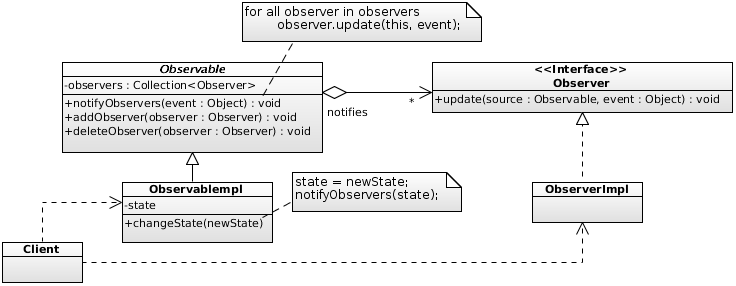
\includegraphics[width=11cm]{observerUml.png}
\caption{UML dell'observer che viene fatto uso direttamente dall'ObservableList}
\label{fig:uml observer}
\end{figure}






\pagestyle{myheadings} 
\markboth{\MakeUppercase{Funzionamento della GUI}}{\MakeUppercase{Funzionamento della GUI}}\chapter*{Funzionamento della GUI}
\addcontentsline{toc}{chapter}{Funzionamento della GUI}
\pagestyle{myheadings}
Il deplyoment è il processo di impacchettamento e distribuzione verso gli utenti del software che abbiamo sviluppato. Si tratta di una parte cruciale del processo di sviluppo poichè costituisce il primo contatto che gli utenti avranno con il nostro software grazie alla quale. \\
L'output può essere sottoformato .exe per gli utenti windows o .dmg per gli utenti os. \\ 
In generale l'impacchettamento .jar è usufruibile per qualunque JVM.
\large
\section*{User-Experience}
\addcontentsline{toc}{section}{User-Experience}
Al lancio dell'applicazione, viene visualizzato un menù realizzato interamente in \textbf{FXML} e \textbf{CSS}. 
La potenzialità di javaFX è di offrire un confortante e immediata interfaccia utente.
\begin{figure}[htp]
\centering
\includegraphics[width=10cm]{1.bmp}
\caption{Inizio}
\label{fig:Inizio}
\end{figure}

Serie di passaggi per effettuare il caricamento da file
\begin{figure}[htp]
\centering
\includegraphics[width=8cm]{2.bmp}
\end{figure}
 
 \begin{figure}[htp]
\centering
\includegraphics[width=8cm]{3.bmp}
\end{figure}

\begin{figure}[htp]
\centering
\includegraphics[width=8cm]{4.bmp}
\end{figure}

\newpage
Il caricamento del file, se è tutto ok, produrrà il dataset nel formato della TableView e verranno visualizzate le possibili checkbox da selezionare. Per ogni checkbox selezionato, sarà evidenziata la corrispondente colonna (grazie all'ObservableList).\\
A questo punto vengono selezionate le Features su cui vogliamo applicare il datamining mediante K-Means, il numero di cluster K e si cliccherà su "Applica K-Means".
\begin{figure}[htp]
\centering
\includegraphics[width=8cm]{5.bmp}
\end{figure}


\begin{figure}[htp]
\centering
\includegraphics[width=8cm]{6.bmp}
\end{figure}

\begin{figure}[htp]
\centering
\includegraphics[width=8cm]{7.bmp}
\end{figure}

\newpage

Se il datamining andrà a buon fine, verrà visualizzato un alert di successo. A questo punto può essere visualizzato il risultato andando a cliccare su "Visualizza Grafico". 
\\ Il grafico che ci si aspetto sarà in 2D poichè si sono scelete solo 2 Features. Si osservi come lo strategy renda trasparente l'intercambiabilità tra il grafico 2D e 3D
\begin{figure}[htp]
\centering
\includegraphics[width=8cm]{8.bmp}
\end{figure}

\begin{figure}[htp]
\centering
\includegraphics[width=8cm]{9.bmp}
\end{figure}

\begin{figure}[htp]
\centering
\includegraphics[width=13cm]{10.bmp}
\caption{Grafico 2D: Osserviamo come i punti siano stati raggruppati, in base al colore, ai loro corrispondenti cluster. Questo visualizzato è un ottimo risultato.}
\label{fig:grafico 2D}
\end{figure}

\newpage
Ora si effettua una prova selezionando 3 features per avere il rsultato finale in un grafico 3D (ci si aspetta il solito lavoro dallo strategy) 
\begin{figure}[htp]
\centering
\includegraphics[width=8cm]{14.bmp}
\end{figure}
\begin{figure}[htp]
\centering
\includegraphics[width=8cm]{16.bmp}
\end{figure}
\begin{figure}[htp]
\centering
\includegraphics[width=10cm]{18.bmp}
\end{figure}
\begin{figure}[htp]
\centering
\includegraphics[width=8cm]{19.bmp}
\end{figure}
\begin{figure}[htp]
\centering
\includegraphics[width=13cm]{20.bmp}
\caption{Grafico 3D: Osserviamo come i punti siano stati raggruppati, in base al colore, ai loro corrispondenti cluster. Anche questo visualizzato è un ottimo risultato. }
\label{fig:grafico 3D}
\end{figure}

\newpage
\large
\section*{Eccezioni: gestione anomalie}
\addcontentsline{toc}{section}{Eccezioni: gestione anomalie}
Osserviamo le eccezioni sviluppato per gestire alcuni eventi anomili.\\
Il k-means potrebbe generare un numero di cluster inferiore a quelli richiesti poichè potrebbero essere scelti dei centroidi "troppo vicini" che non riescono a creare il gruppo di cluster.
\begin{figure}[htp]
\centering
\includegraphics[width=10cm]{13.bmp}
\caption{Errore del kmeans. L'eccezione lanciata è "AlgoritmoDivergenteException".}
\label{fig:ecc kmeans}
\end{figure}

Il numero delle features devono essere almeno due, altrimenti il datamining non avrebbe senso.
\begin{figure}[htp]
\centering
\includegraphics[width=10cm]{26.bmp}
\caption{Errore selezione features.L'eccezione lanciata è "FeatureInsufficientiException"}
\label{fig:sel feu}
\end{figure}

\newpage
Caso in cui si hanno errori sulla reperibilità del file
\begin{figure}[htp]
\centering
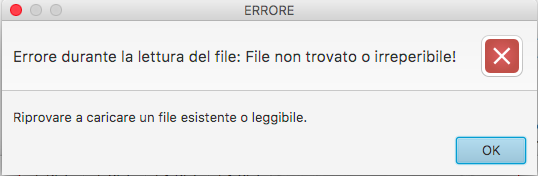
\includegraphics[width=10cm]{30.png}
\caption{Errore apertura file.L'eccezione lanciata è "FileNonTrovatoException"}
\label{fig:sel feu}
\end{figure}
Il file non è formato da valori adeguati (solo numeri).
\begin{figure}[htp]
\centering
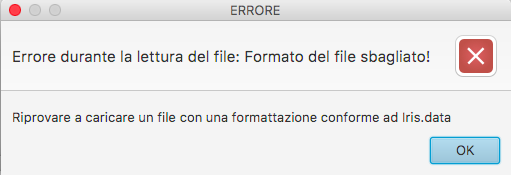
\includegraphics[width=10cm]{31.png}
\caption{Errore formato interno file.L'eccezione lanciata è "FileNumeriFormatoException"}
\label{fig:sel feu}
\end{figure}




\pagestyle{myheadings} 
\markboth{\MakeUppercase{Bibliografia e strumenti di sviluppo}}{\MakeUppercase{Bibliografia e strumenti di sviluppo}}\chapter*{Bibliografia e strumenti di sviluppo}
\addcontentsline{toc}{chapter}{Bibliografia e strumenti di sviluppo}
\pagestyle{myheadings} 

La seguente relazione è stata realizata in {\LaTeX} utilizzando l'omonimo linguaggio ed è stato utilizzato SublimeText come editor poichè si è utilizzato un Macbook.
\begin{description}
\item [Fonte di studio] 
        \begin{itemize}
            \item Slide del corso di di programmazione 3
            \item Manuale di Java di Claudio De Sio
            \item Getting Started with JavaFX
            \item Object Oriented Design
        \end{itemize} 
\item [Strumento hardware di sviluppo] Macbook Air 2015.
\item [Software usati per la progettazione di schemi]  ObjectAid UML Explorer.
\item [IDEE e ambiente di sviluppo] IDE: Eclipse Mars.1 plugin: e(fx)clipse.
\end{description} 
 \end{document}